% lutorch_ex library report (DRAFT — to be refined). Build: latexmk -pdf -interaction=nonstopmode lutorch_ex_report.tex
% Style/preamble adapted from doc/research/lut_ablation/lut_ablation_table_v4.tex.
% SOURCES: doc/lutorch/lut_mechanisms.tex (cartridge math), doc/research/lut_ablation/lut_ablation_table_v4.tex
%          (ablation results), sources/quantisation_simple_norowops.md (quant math), src/spiky/lutorch_ex/ (code).
\documentclass[11pt]{article}
\usepackage[margin=1in]{geometry}
\usepackage{lmodern}
\usepackage[T1]{fontenc}
\usepackage{amsmath,amssymb}
\usepackage{booktabs,longtable,array}
\usepackage{xcolor}
\usepackage{listings}
\usepackage{tikz}
\usetikzlibrary{positioning,arrows.meta,backgrounds,fit,calc}
\usepackage{hyperref}
\hypersetup{colorlinks=true,linkcolor=black,urlcolor=blue}

\newcommand{\tbd}[1]{\textcolor{red!70!black}{\textbf{[TBD}~--- #1\textbf{]}}}
\newcommand{\code}[1]{\texttt{#1}}
\newcommand{\sgn}{\operatorname{sgn}}
\lstset{basicstyle=\ttfamily\small,columns=fullflexible,breaklines=true,frame=single,language=Python,
        keywordstyle=\color{blue!60!black},commentstyle=\color{green!40!black},showstringspaces=false}

\title{\textbf{The \code{lutorch\_ex} library}\\[2pt]\large lookup-table FFNs: tables, projections, cartridges, and results}
\author{(draft)}
\date{2026-10-05 (DRAFT — refine next session)}

\begin{document}
\maketitle

% ======================================================================================================
\section{The basic idea: lookup tables over an LSH}
\label{sec:idea}

A lookup table (LUT), here, is a learnable map built from a \emph{discrete} address: hash the input to a small
integer with a locality-sensitive hash (LSH), and read a stored vector at that address. The hash is cheap --- a
handful of sign bits --- so a ``read'' is a gather plus a few adds, not a matrix multiply. \code{lutorch\_ex}
builds many such tables and sums them into an expressive learnable map. This is a general construction; using it
as a drop-in feed-forward layer (the setting benchmarked in \S\ref{sec:ml}) is just one application of it, not
its defining purpose.

\paragraph{One table.} Work in a per-head space $z\in\mathbb{R}^{d_\text{in}}$. A table picks \code{nap}
\emph{anchors}, each defining one scalar form $u_j$ of $z$; the \emph{signs} of the $u_j$ form an
\code{nap}-bit address $c\in[0,K)$ into $K=2^{\text{nap}}$ cells, and each cell holds a learnable vector
$W[c]\in\mathbb{R}^{d_\text{out}}$. Each sign bit is one LSH bit --- which side of a hyperplane $u_j=0$ the
input lies on; inputs on the same side of all \code{nap} hyperplanes share a cell. The margins $u_j$ (how far
each form is from flipping its sign) measure the address's confidence --- a small margin means a bit is near
its boundary.

\paragraph{Primitive hyperplanes only (at the cartridge level).} The hyperplanes a cartridge can use are
deliberately \emph{primitive}: each passes through the origin (zero bias) and has trivial coefficients. Two
modes:
\begin{itemize}
\item \textbf{pairs} (\code{anchor\_mode="pairs"}): $u_j = z[a_j]-z[b_j]$ --- coefficients in $\{-1,+1\}$ on two
  coordinates (the \emph{anchor pairs}).
\item \textbf{single} (\code{anchor\_mode="single"}): $u_j = z[a_j]$ --- a single $+1$ coefficient (the even
  simpler \emph{single anchors}), so the bit is just the sign of one coordinate.
\end{itemize}
Both share the same read; only how the \code{nap} forms are built changes. Crucially, \emph{arbitrary}
hyperplanes ($w^\top z$ with general $w$ and bias) are \textbf{not} available at the cartridge level --- that is
exactly what \S\ref{sec:projection}'s input projection provides: a learned Linear maps the input first, and the
primitive $\{-1,+1\}$/single-coordinate hashing is then applied in the projected space, so a primitive form on
$\text{compress}(x)$ realises an arbitrary learned hyperplane on $x$.

\paragraph{Many tables, many heads.} The layer stacks \code{tph} tables per head over $G$ head-groups
($G=\code{n\_groups}=\max(h_\text{in},h_\text{out})$). A head's read \emph{sums} the addressed cell(s) over its
\code{tph} tables (optionally weighted --- see the cartridges), giving a per-group output
$[B,G,d_\text{out}]$, which a routing step maps to $[B,h_\text{out},d_\text{out}]$ (identity when
$h_\text{out}=G$; a group-sum when $h_\text{out}=1$).

\paragraph{Geometry and the base.} The immutable geometry is \code{LUTSpec}: \code{h\_in, h\_out, tph, nap,
d\_in, d\_out}, with \code{n\_cells}$=2^{\text{nap}}$, \code{in\_features}$=h_\text{in}d_\text{in}$,
\code{out\_features}$=h_\text{out}d_\text{out}$. The abstract base \code{ManifestoLUT} owns the learnable cell
tables $W\in\mathbb{R}^{G\times\text{tph}\times K\times d_\text{out}}$ and the addressing (\code{\_addresses},
which uses only spec/anchors/powers --- never the weight \emph{values}), the routing invariant
(\code{\_route}), and the cell total-variation penalty (\S\ref{sec:reg}). The faithful default init draws cell
tables per head from a CPU generator seeded $(\text{seed}+h+1)$, $\text{Uniform}[-\sigma,\sigma]$ with
$\sigma=\code{weight\_init\_std}$ (realised std $\sigma/\sqrt3\approx5.8\mathrm{e}{-4}$ at the $10^{-3}$
default), reproducing the OLD LightMHL draw bit-for-bit.

% ======================================================================================================
\section{ProjectionLUT: input and output projections}
\label{sec:projection}

\begin{figure}[t]
\centering
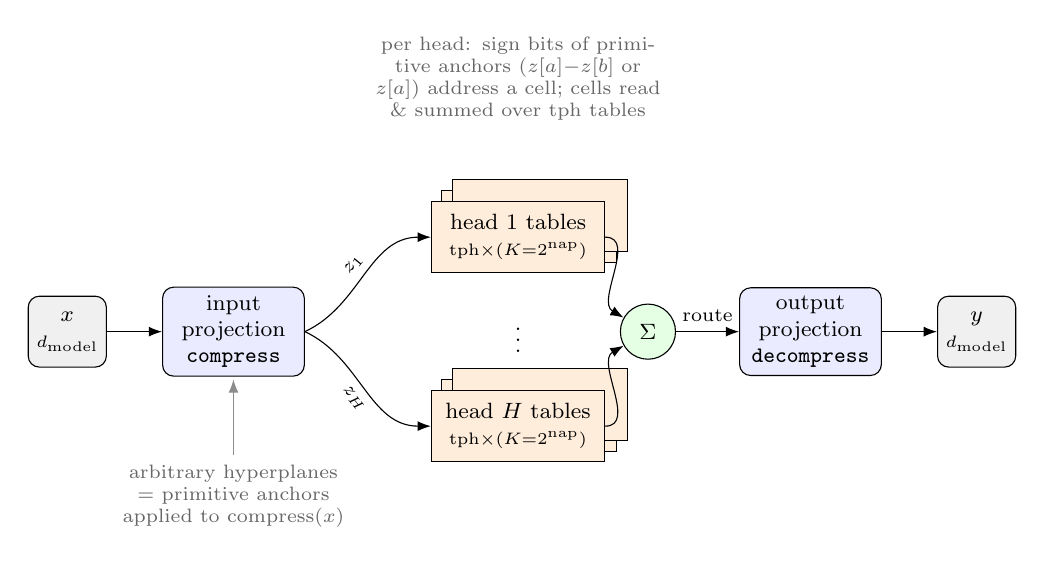
\begin{tikzpicture}[>=Latex, font=\footnotesize,
  box/.style={draw, rounded corners, align=center, inner sep=3pt, minimum height=9mm},
  io/.style={box, fill=black!6},
  proj/.style={box, fill=blue!8, minimum width=18mm},
  tbl/.style={draw, fill=orange!14, align=center, inner sep=3pt, minimum width=22mm, minimum height=9mm},
  sumop/.style={draw, circle, inner sep=1pt, minimum size=7mm, fill=green!10}]
\node[io] (x) {$x$\\$\scriptstyle d_\text{model}$};
\node[proj, right=7mm of x] (cmp) {input\\projection\\\code{compress}};
\node[tbl, right=16mm of cmp, yshift=12mm] (t1) {head $1$ tables\\$\scriptstyle \text{tph}\times(K{=}2^{\text{nap}})$};
\node[tbl, right=16mm of cmp, yshift=-12mm] (t2) {head $H$ tables\\$\scriptstyle \text{tph}\times(K{=}2^{\text{nap}})$};
\node at ($(t1)!0.5!(t2)$) {$\vdots$};
\node[sumop, right=16mm of cmp, xshift=24mm] (sum) {$\Sigma$};
\node[proj, right=8mm of sum] (dec) {output\\projection\\\code{decompress}};
\node[io, right=7mm of dec] (y) {$y$\\$\scriptstyle d_\text{model}$};
% stack effect (multiple tables per head)
\begin{scope}[on background layer]
  \foreach \t in {t1,t2}{ \foreach \dx in {1.4,2.8}{
    \draw[fill=orange!14, draw=black] ([xshift=\dx mm,yshift=\dx mm]\t.south east) rectangle ([xshift=\dx mm,yshift=\dx mm]\t.north west); }}
\end{scope}
\draw[->] (x) -- (cmp);
\draw[->] (cmp.east) to[out=25,in=180] node[above,sloped,font=\scriptsize]{$z_1$} (t1.west);
\draw[->] (cmp.east) to[out=-25,in=180] node[below,sloped,font=\scriptsize]{$z_H$} (t2.west);
\draw[->] (t1.east) to[out=0,in=150] (sum);
\draw[->] (t2.east) to[out=0,in=210] (sum);
\draw[->] (sum) -- node[above,font=\scriptsize]{route} (dec);
\draw[->] (dec) -- (y);
\node[below=10mm of cmp.south, text width=34mm, align=center, font=\scriptsize, text=black!60] (cn)
  {arbitrary hyperplanes = primitive anchors applied to $\mathrm{compress}(x)$};
\draw[->, black!45, shorten >=1pt] (cn) -- (cmp);
\node[above=9mm of $(t1.north)$, text width=46mm, align=center, font=\scriptsize, text=black!60] (an)
  {per head: sign bits of primitive anchors ($z[a]{-}z[b]$ or $z[a]$) address a cell; cells read \& summed over tph tables};
\end{tikzpicture}
\caption{The ProjectionLUT data path. The input $x$ is projected by \code{compress} into $H$ per-head spaces;
each head's primitive-anchor LSH addresses its own stack of \code{tph} discrete tables ($K=2^{\text{nap}}$ cells
each); the per-head reads are summed and routed, then \code{decompress} projects back to $y$. Only the input
projection realises arbitrary hyperplanes --- the cartridge itself sees primitive $\{-1,+1\}$/single-coordinate
anchors with zero bias.}
\label{fig:projlut}
\end{figure}

On its own a table reads a narrow per-head vector. \code{ProjectionMHL} (the ``ProjectionLUT'' wrapper, drawn in
Figure~\ref{fig:projlut}) turns a cartridge into a plain $d_\text{model}\!\to\!d_\text{model}$ FFN with a linear
map on each side, for two reasons:
\begin{itemize}
\item \textbf{input projection (\code{compress})} --- a Linear $d_\text{model}\!\to\!\code{in\_features}$ learns
  the coordinates the hash reads, i.e.\ it \emph{shapes the hashing} so the sign bits fall where they carry
  signal, instead of hashing raw model dimensions.
\item \textbf{output projection (\code{decompress})} --- a Linear $\code{out\_features}\!\to\!d_\text{model}$
  lets the tables live in a narrow $d_\text{out}$ space and be \emph{compressed}: the cells are small, and the
  projection expands the summed read back to model width.
\end{itemize}
The forward is $z=\text{compress}(x)$ (reshaped to $[B,h_\text{in},d_\text{in}]$); $y=\text{cartridge}(z)$;
$\text{out}=\text{decompress}(y)$. Either side may be switched off (Identity) when the widths already match.

\paragraph{Init and first-backward warmup.} \code{compress}$\sim\mathcal N(0,0.02)$; \code{decompress} is
\emph{zeroed}. Since $\partial\,\text{out}/\partial y=W_\text{dec}=0$ at init, the first backward sends no
main-loss gradient to the cartridge or \code{compress}; only \code{decompress} (and the tables, via the TV
term) move on step 0, and the input side ``warms up'' once \code{decompress} leaves zero --- reproducing OLD's
zero-contribution FFN at init. Both inits are meta-guarded so the deployment skeleton allocates nothing.

\paragraph{Two capabilities it mediates.} (i) \code{SupportsDecompressBake}: a cartridge may expose
\code{decompress\_scale()} (length \code{out\_features}); \code{ProjectionMHL} folds it into the
\code{decompress} matrix on every forward (scaling column $k$ $=$ scaling cartridge output channel $k$, no extra
op) --- the route by which a quantised cartridge's per-channel scale moves into the dense projection. (ii)
\code{SupportsDeploymentExport}: \code{to\_deployment()} for compaction, used by the deployment path
(\S\ref{sec:arch}); \code{ProjectionMHL} is the seam where the power-of-two scale is folded into
\code{decompress}, once, at export.

% ======================================================================================================
\section{Cartridges: different math, one contract}
\label{sec:cartridges}

Everything above is fixed: the geometry, the addressing, the per-head sum, the routing, the projection wrapper.
A \emph{cartridge} is the swappable lookup \emph{math} that sits inside that contract --- how a table turns its
addressed cell(s) and margins into an output. All cartridges share the read skeleton (each group addresses one
cell $c_g$ per table from the sign pattern, the read sums over the \code{tph} tables, then \code{\_route}s
$[B,G,d_\text{out}]\!\to\![B,h_\text{out},d_\text{out}]$); they differ in whether the read is hard or blended,
whether it is weighted by a learned confidence score, and whether it is quantised. The next section covers each.
\tbd{cross-check the finer per-cartridge forms against \code{doc/lutorch/lut\_mechanisms.tex} (\S LightMHL, \S
confidence forms, \S Gen-2 soft-sign).}

% ======================================================================================================
\section{The cartridges}
\label{sec:body}

\subsection{\code{ConfidenceLUT}}
Gen-3 scored read. A learned-margin confidence score weights each table's cell contribution. With margins
$u$ and $m=|u|$, the per-table score is
\[
 s \;=\; \Big(\textstyle\sum_j m_j\Big)\,\exp\!\Big(\gamma\textstyle\sum_j \log\sigma(\beta\,m_j)\Big),
\]
$\beta=e^{\log\beta}$, $\gamma=e^{\log\gamma}$ learnable (per layer; $g$ frozen at $0$ in the champion). A large
score means every margin is large, i.e.\ the address is confident. The $n{=}2$ read blends the addressed cell
$c_1$ and the runner-up $c_2$ (flip the least-certain bit, the smallest margin $u^\star=\min_j u_j$) with a
softmax over the deciding margin: $v=\sigma(2u^\star/\tau)$, contributing $s\,[\,v\,W[c_1]+(1-v)\,W[c_2]\,]$;
$n{=}1$ reads only the scored cell $s\,W[c_1]$. Gradients flow to $W$, $\beta$, $\gamma$ (and $\tau$ for $n{=}2$).
\begin{lstlisting}
from spiky.lutorch_ex import LUTSpec, ConfidenceLUT, ProjectionMHL
spec = LUTSpec(h_in=8, h_out=8, tph=64, nap=8, d_in=48, d_out=48)
cart = ConfidenceLUT(spec, seed=1, read_top_n=2, beta_init=2.0, gamma_init=1.0,
                     read_tau_init=0.5, read_tau_learnable=True)
ffn  = ProjectionMHL(cart, d_model=384)   # drop-in d_model -> d_model FFN
\end{lstlisting}

\subsection{\code{QuantisedConfidenceLUT} (extended)}
The p2\_int8 quant-aware twin of \code{ConfidenceLUT}. Same confidence score/blend, but the read is
quantisation-aware with a straight-through estimator (STE):
\begin{itemize}
\item \textbf{Cell tables} are fake-quantised to int8 with a per-(group,channel) \emph{power-of-two} scale:
 for group $g$, channel $k$, an integer exponent $e_{g,k}$ (\code{head\_chan\_exponents}) gives
 $\hat W = \mathrm{round}(W/2^{e})\cdot 2^{e}$, clamped to int8; STE passes the identity gradient to the fp32
 master $W$.
\item \textbf{Blend weights} are rounded to powers of two: $2^{k'}$ and $2^{k'-q}$ with
 $k'=\mathrm{round}(\log_2 s - c_q)$ and $q=\mathrm{round}(2|u^\star|/(\tau\ln 2))$ (stop-grad exponents;
 the STE carries the exact $(s\!\cdot\!v,\,s\!\cdot\!(1\!-\!v))/s$ gradient).
\item \textbf{Integer read} (\code{forward\_int} / the deployed path): int8 cell rows, int32 shift-add in fixed
 point (shift $=6$, \code{FIXED\_POINT\_SHIFT}), accumulator in units $2^{-6}$, then scaled by $2^{\,e-6}$ per
 (group,channel). Equals the fake-quant forward value to round-off.
\end{itemize}
\textbf{Deployment bake.} \code{to\_deployment()} emits the int8 \code{packed} table and the per-out-feature
scale $2^{\,e-6}$; \code{export\_deployment} folds that pure-power-of-two multiplier \emph{exactly} into a copy
of the \code{decompress} weight (scaling column $k$ by $2^{\,e-6}$ only touches the fp32 exponent field). The
deployed cartridge returns the \emph{raw} int32 accumulator and reports \code{decompress\_scale()}$=$None (the
scale is static in the stored weight). Requires \code{read\_top\_n}$=2$ and $h_\text{out}=G$ (the champion);
fan-in would need a pre-route scale.

\textbf{Exact constants} (from \code{sources/quantisation\_simple\_norowops.md}). \code{quant\_cfg}: $b=8$ bits,
offset $o=0$. Blend: $q=\mathrm{clamp}\!\big(\lfloor 2u^\star/(\tau\ln 2)+\tfrac12\rfloor,0,J\big)$ with $J=64$,
$c_q=\log_2(1+2^{-q})$ for $q<C=8$ (else $0$); the second cell is dropped when $q>Q=3$. The weight exponent
$k'=\mathrm{round}(\log_2 s-c_q)$ lives in an $L=8$ window $[-3,4]$ ($k_\text{max}=4$, 3 bits): $k'<-3$ skips the
table (weight 0, gradient kept), $k'>4$ clamps (fires on $\sim$0.001--0.007\% of tables). The per-(head,channel)
weight exponent is $e_{h,c}=\big\lceil\log_2\max_{t\in h,\,\text{cells}}|W_t[\cdot]_c|\big\rceil-(b-1)+o$ --- the
max over the \emph{head's} tables, so one exponent is shared across them (int8 $o=0$, never saturates; int4
$b=4,o=-1$). \code{FIXED\_POINT\_SHIFT}$=6$ because $k'+6\ge0$ and $k'+6-q\ge0$ for all $k'\ge-3,\,q\le3$, so
the integer read is pure left-shifts-and-adds. The decompress fold is exact precisely because $e_{h,c}$ is
shared across a head's tables (it factors out of the table sum) \emph{and} nothing sits between the table sum
and \code{decompress}. Measured cost: $\sim$+0.003\,bpb vs the unquantised soft read; footprint 151.0\,MB fp32
$\to$ 37.75\,MB int8 ($4\times$) $\to$ 18.87\,MB int4 ($8\times$).
\begin{lstlisting}
from spiky.lutorch_ex import QuantisedConfidenceLUT, ProjectionMHL, export_deployment, load_deployment
cart = QuantisedConfidenceLUT(spec, seed=1, quant_mode="p2_int8", read_top_n=2,
                              beta_init=2.0, gamma_init=1.0, read_tau_init=0.5)
ffn  = ProjectionMHL(cart, d_model=384)
# ... train ...
export_deployment(model, "m.lxq")                      # int8 bake + fold pow2 scale into decompress
dep = load_deployment("m.lxq", make_skeleton, device="cuda").eval()   # fp32 table never allocated
\end{lstlisting}

\subsection{\code{FusedManifestoHardLUT}}
Hard value read $\sum_t W[c_t]$ (the argmax cell per table, no score weighting), fused. The tier-2 native path
uses the lprojection non-smooth backward; tier-1 fuses the per-table gather + sum with \code{embedding\_bag}.
\tbd{exact forward/backward from \code{manifesto\_hard.py} + \code{\_native\_ops.NativeHard}.}
\begin{lstlisting}
from spiky.lutorch_ex import FusedManifestoHardLUT, ProjectionMHL
ffn = ProjectionMHL(FusedManifestoHardLUT(spec, seed=1), d_model=384)
\end{lstlisting}

\subsection{\code{FusedManifestoSoftLUT}}
Soft temperature-blended read; the native path uses \code{lprojection\_forward\_smooth} and its na1-smooth
backward. \tbd{soft-blend math from \code{manifesto\_soft.py}.}

\subsection{\code{FusedSoftSignHardLUT} / \code{FusedSoftSignSmoothLUT}}
Gen-2 soft-sign cartridges. The two-cell blend weight is $w=\sigma(-2\rho/T_\text{sel})$ with
$\rho=|m|/(T_\text{soft}+|m|)$ (deciding margin $m$, learned temperatures $T_\text{soft},T_\text{sel}$); the
hard variant uses the straight-through value, the smooth one the true blend. The surrogate's $m$/$T$ gradients
are a one-launch \code{softsign\_surrogate\_grad} kernel (tier-1: eager). \tbd{confirm against
\code{softsign\_*.py} + \code{\_native\_softsign.py}; lut\_mechanisms has the Gen-2 forms.}
\begin{lstlisting}
from spiky.lutorch_ex import FusedSoftSignHardLUT, FusedSoftSignSmoothLUT, ProjectionMHL
ffn = ProjectionMHL(FusedSoftSignSmoothLUT(spec, seed=1), d_model=384)
\end{lstlisting}

% ======================================================================================================
\section{Experiments}
\label{sec:ml}

\subsection{Architecture and implementation}
\label{sec:arch}
The experiments drop a \code{ProjectionLUT} FFN into every block of a small GPT (6 blocks, model width
$d_\text{model}=384$, $\approx$68.2M params). Two implementation notes. \emph{Native-op resolution:} the fused
cartridges reach a tier-2 CUDA fast path through one choke point, \code{\_native\_ops.native\_manager()}, which
resolves (1) the co-located JIT extension \code{lutorch\_ex\_lprojection} (vendored lprojection / anchor-pairs
kernels, built from \code{cartridges/csrc/} via \code{cpp\_extension.load}), then (2) the pure/tier-1 torch
path; the int8 read is a second JIT extension, \code{lutorch\_ex\_pow2\_int8\_read}. \emph{Deployment:}
\code{export\_deployment}/\code{load\_deployment} write and load a compact, cartridge-agnostic \code{.lxq}
safetensors checkpoint --- \code{make\_skeleton} builds on the \code{meta} device (no fp32 allocation) and each
compacted FFN is rebuilt from a stored format tag via the leaf \code{deploy\_registry}, so the fp32 LUT table is
never allocated and the quantised footprint drops $\sim$4$\times$.

\subsection{Regularisation and training recipe}
\label{sec:reg}
Two regularisers are part of the champion recipe (applied on \code{lutorch\_ex}, not the skeleton).

\paragraph{Cell total-variation ($\mathcal R_\text{TV}$, $\lambda=10$).} View each table's $K=2^\text{nap}$
cells as the vertices of an nap-dimensional hypercube
($[\,G\!\cdot\!\text{tph},\,\underbrace{2,\dots,2}_{\text{nap}},\,d_\text{out}\,]$). The penalty sums the squared
difference (channels summed in) over every Hamming-1 cell pair --- a size-2 \code{diff} along each of the nap
bit-axes, each pair counted once --- normalised by the pair count:
\[
 \mathcal R_\text{TV} \;=\; \frac{1}{n_\text{tables}\,\text{nap}\,2^{\text{nap}-1}}
   \sum_{\substack{(c,c')\ \text{Hamming-1}}} \bigl\lVert W_c - W_{c'}\bigr\rVert_2^2 .
\]
Added to the loss as $\lambda\,\mathcal R_\text{TV}$ ($\lambda=10$) through a separate backward; differentiable
w.r.t.\ $W$ only; adds nothing to the forward. Hamming-1 neighbours are addressed by inputs differing in a
single anchor-sign bit, so penalising their squared difference smooths the table --- a one-bit address flip
changes the read little (a locality prior over the discrete lookup). (Bit-for-bit the reference
\code{LightMultiHeadLUT.cell\_tv}.)

\paragraph{Head (table) dropout ($r=0.2$).} Inverted dropout at whole-table granularity: one independent
Bernoulli per (sample, group$=$head, table) on $[B,G,\text{tph}]$, keep prob $1-r$, survivors rescaled
$1/(1-r)$; dropped tables contribute $0$. Train-time + grad-only (eval reads all tables); the same keep-mask
multiplies the backward. It discourages co-adaptation among a head's \code{tph} tables.

\paragraph{Hyperparameters.} All seven runs share the champion topology ($h{=}8$, \code{tph}$=64$,
\code{nap}$=8$, $d_\text{in}=d_\text{out}=48$, $d_\text{model}=384$), seed 1, faithful small-std init, cell-TV
$\lambda=10$, head-dropout $0.2$. Training: AdamW lr $3\!\times\!10^{-4}$, weight decay $0.1$ (none on the LUT
tables), $48{,}000$ steps, cosine schedule ($10\%$ warmup, $0.1\times$ floor), sequence length $512$, device
batch $12$, total batch $24{,}576$ tokens, eval every $500$. wandb project \code{Spiky}, group
\code{lutorch\_ex}; per-run artifacts (config, metrics, summary) are under \code{experiments/lutorch\_ex/}.

\subsection{The seven-config sweep}
All seven runs are complete. Final \code{val\_bpb} (best$\to$worst):

\begin{longtable}{@{}l l l r@{}}
\toprule
Configuration & cartridge / mode & wandb run & final \code{val\_bpb} \\
\midrule
ConfidenceLUT $n{=}2$        & scored, float          & \code{lutorch\_ex\_abl47\_conf\_1004\_1148}            & \textbf{1.10606} \\
QuantConfidence $n{=}2$      & scored, p2\_int8       & \code{lutorch\_ex\_abl47\_quant\_1004\_1148}           & 1.10724 \\
ConfidenceLUT $n{=}1$        & scored, float, $n{=}1$ & \code{lutorch\_ex\_abl47\_conf\_n1\_vm\_1004\_1806}    & 1.11737 \\
FusedSoftSignSmooth         & soft-sign, smooth      & \code{lutorch\_ex\_abl47\_fss\_smooth\_vm\_1004\_1806} & 1.12941 \\
FusedManifestoSoft          & soft                   & \code{lutorch\_ex\_abl47\_fms\_wk\_1004\_1510}         & 1.13949 \\
FusedManifestoHard          & hard                   & \code{lutorch\_ex\_abl47\_fmh\_wk\_1004\_1510}         & 1.15152 \\
FusedSoftSignHard           & soft-sign, hard        & \code{lutorch\_ex\_abl47\_fss\_hard\_wk\_1004\_1510}   & 1.15647 \\
\bottomrule
\end{longtable}

\paragraph{Reading the results.} The scored \code{ConfidenceLUT} line wins: $n{=}2$ is best at
\textbf{1.10606}, and int8 power-of-two quantisation of it costs only $+0.0012$ bpb (1.10724) --- consistent
with the reference's $\sim$+0.003 bpb upper bound --- for a $4\times$ smaller table. Dropping the blend to a
single cell ($n{=}1$) costs $+0.0113$. The non-scored families trail: the soft reads (FusedSoftSignSmooth
1.12941, FusedManifestoSoft 1.13949) beat their hard counterparts (FusedManifestoHard 1.15152, FusedSoftSignHard
1.15647). So a soft/blended read and a learned confidence score each help, and they stack.

\paragraph{Learning curves.} \tbd{insert the \code{val\_bpb} learning-curve figure (7 curves); data is in
\code{experiments/lutorch\_ex/*/metrics.csv}.}

\end{document}
